\section{DALILA}\label{codesec}
DALILA is a library for signal decomposition and reconstruction. Its first focus is Dictionary Learning (DL) described in Section \ref{background}. The fact that both the dictionary and the coefficients are learned from data allows for a more complete analysis of the results  extracting useful information about the original signals. Moreover the possibility to impose prior knowledge on the problem using penalty terms grants that the final matrices respect certain constraints.
Examples for regularised DL are: 1) image denoising where sparsity imposition forces the most important atoms to be used and the noisy ones to be discarded; 2) pattern recognition, where the atoms of the dictionary are seen as latent patterns from which the original signals are generated.

DALILA second focus is Representation Learning whose purpose is to represent the original data matrix on a new space defined by the atoms of the dictionary $\mathbf{D}$. Penalty terms can be added to impose a structure on this new representation.

The learned coefficients may be used as a new representation for further tasks such as: 1) compressed sensing that exploits sparsity reducing the size of the original signal; 2) classification where, rather than considering the original signal, the coefficients are used as new features.

\begin{figure}[!h]
\centering
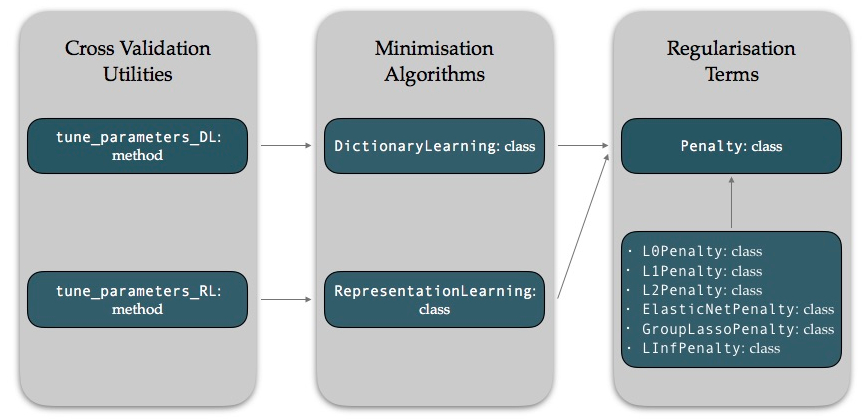
\includegraphics[width=0.9\textwidth]{schema}
\caption{Diagram of DALILA library structure.
The main core consists of the two classes which address the minimization problem.
This depends on the class Penalty which represents a generic penalty term and that can be specialised by declaring subclasses.
 The library also offers cross validation utilities for the free parameters tuning. }
\label{schema}
\end{figure}

\subsection{Implementation}
DALILA is implemented in Python. It supports different versions of Python and it is \texttt{scikit-learn} compatible. See \url{https://slipguru.github.io/dalila} for the full documentation and a quick start.

DALILA has a modular and easily extendible design (see Figure \ref{schema}). The core of the library consists of two classes,  \texttt{DictionaryLearning} and \texttt{RepresentationLearning} which respectively solve the two minimisation problems in Equation (\ref{generic functional}) and (\ref{sparse coding}). These classes depend on a generic penalty term (\texttt{Penalty}) which can be specialised into different regularisers by declaring a subclass. The library is therefore easily extendible with new regularisers and flexible in the choice of the model.
Cross validation utilities to tune the parameters of the model are provided, the two methods shown in Figure \ref{schema}, \texttt{tune\_parameters\_DL} and \texttt{tune\_parameters\_RL}, can perform the tuning by parallel or distributed computation using \texttt{dask} library \cite{dask}.\\

%\textcolor{red}{In the library the loss function $\ell$, introduced in a generic form in Equation (\ref{generic functional}) and (\ref{sparse coding}), is commong to both \texttt{DictionaryLearning} and \texttt{RepresentationLearning} classes and it is the Frobenius norm of the difference between the original signal and its reconstruction, defined as Equation (\ref{square loss}).}

The loss function $\ell$ introduced in a generic form in Equation (\ref{generic functional}) and (\ref{sparse coding}) is common to both \texttt{DictionaryLearning} and \texttt{RepresentationLearning} classes.
It is implemented as the Frobenius norm of the difference between the original signal and its reconstruction, defined as Equation (\ref{square loss}).
\begin{equation}\label{square loss}
\ell(\textbf{X}, \textbf{CD}) = \|\textbf{X} - \textbf{CD}\|_F^2
\end{equation}

As regards the regularisation terms, called $\Phi$ and $\Psi$ in Equation (\ref{generic functional}) and (\ref{sparse coding}),  DALILA
offers many possibilities.
%The implementation of %as \texttt{L1Penalty}, \texttt{L2Penalty}, \texttt{ElasticNetPenalty}, \texttt{GroupLassoPenalty},
%\texttt{LInfPenalty} and \texttt{L0Penalty} (described in Section \ref{penaltiessec}) is provided.
In this way a proper regulariser, dependent from the task, can be chosen, during the initialisation of the \texttt{DictionaryLearning/RepresentationLearning} instances.
In fact \texttt{DictionaryLearning/RepresentationLearning} minimisation algorithms do not depend on the penalties chosen,
as long as the penalty classes inherit from the superclass \texttt{Penalty} and reimplement the same methods (Figure \ref{schema}).
For a better understanding see Appendices \ref{penalty change}, \ref{new penalty}.
\paragraph*{Available regularisation terms}\label{penaltiessec}
%\textcolor{red}{The penalty terms in the library refer to the ones introduces in Equation (\ref{generic functional}) and (\ref{sparse coding}), $\Phi$ and $\Psi$. We now explain some of the possible choices and their properties.}

The penalty terms $\Phi$ and $\Psi$ are the product between a regularisation parameter and, typically, a norm. The norm is used to impose a structure on the matrix, while the regularisation parameter, a positive scalar, weights the regularisation term influence on the solution.%regularised the solution should be.
%All the penalties we present here are applied by row because of the structure of the matrices: on the rows of coefficients matrix lie the samples while on the rows of the dictionary matrix lie the atoms.

In the following we show the possible choices for $\Phi$ and $\Psi$ applied on a generic matrix $\textbf{M}$ whose $i$-th row is indicated as $\textbf{M}_{i,:}$ and $j$-th column as $\textbf{M}_{:,j}$. Its generic element is denoted by $m_{ij}$. With the notation $\Phi|\Psi$ we indicate that the penalty can be applied or on the dictionary or on the coefficients or on both.\\
\begin{itemize}
%
%
%
\item \texttt{L1Penalty} - \textbf{$\ell_1$ norm}
\begin{equation}\label{l1penalty}
\Phi|\Psi(\mathbf{M}) = \lambda \sum_i \|\mathbf{M}_{i,:}\|_1 =  \lambda \sum_i \sum_j |m_{ij}|
\end{equation}
Regularisation terms of this form, due to the geometrical meaning of the $\ell_1$ norm, force the solution to be sparse and, therefore, highly interpretable \cite{tibshirani1996regression}. If the penalty is applied on the dictionary it promotes a dictionary whose atoms have a low number of non-null components. For the coefficients, the penalisation promotes a reconstruction based only on few atoms of the dictionary, discarding the ones which give minor contribution to the original signal.

The proximal operator related to this regulariser is
\begin{equation}\label{proxl1}
\text{prox}_{\Phi|\Psi}(m_{ij}) =
\begin{cases}
       m_{ij} - \lambda &\text{ if }m_{ij} > \lambda \\
       0 & \text{ if }m_{ij} \in [-\lambda, \lambda] \\
       m_{ij} + \lambda & \text{ if }m_{ij} < -\lambda
\end{cases}
\end{equation}
%
%
%
\item \texttt{L2Penalty} - \textbf{$\ell_2$ norm}
\begin{equation}\label{l2penalty}
\Phi|\Psi(\mathbf{M}) = \lambda \sum_{i}\left({\sum_j m_{ij}^2}\right)^\frac12
\end{equation}

Penalties of this form, as in the previous case, can be applied to both matrices $\mathbf{C}$ and $\mathbf{D}$.
The $\ell_2$ regularisation term leads to the shrinkage of the components of each row, but, differently from the $\ell_1$ norm, it does not lead to a sparse solution \cite{tikhonov1977solutions}.

The proximal operator is
\begin{equation}\label{proxl2}
\text{prox}_{\Phi|\Psi}(\mathbf{M}_{i,:}) = \text{max}(1 - \lambda/ \| \mathbf{M}_{i,:}\|_2, 0)\ \mathbf{M}_{i,:}
\end{equation}
%
%
%
\item \texttt{ElasticNetPenalty}
\begin{equation}\label{l1l2penalty}
\Phi|\Psi(\mathbf{M}) = \sum_{i}\bigg[\alpha \lambda_1 \|\mathbf{M}_{i,:}\|_1 + (1 - \alpha)\lambda_2 \|\mathbf{M}_{i,:}\|_2 \bigg]
\end{equation}
Elastic Net can be preferable to $\ell_1$ norm, in the case of highly correlated variables, and also to $\ell_2$ norm since it inherits the possibility of finding a sparse solution \cite{zou2005regularization}.

Here $\lambda_1$ and $\lambda_2$ weight the two norms separately while $\alpha \in [0,1]$ balances the contribution of the two terms. The proximal operator is

\begin{equation}\label{proxen}
\text{prox}_{\Phi|\Psi}( \mathbf{M}_{i,:}) = \left(\frac{1}{1 + \alpha\lambda_2}\right) \text{prox}_{\lambda_1 \|\cdot\|_1} ( \mathbf{M}_{i,:})
\end{equation}
%
%
\item \texttt{L0Penalty} - \textbf{$\ell_0$ pseudo-norm}
\begin{equation}\label{l0penalty}
\Phi|\Psi(\mathbf{M}) : \forall i\ \    \|\mathbf{M}_{i,:}\|_0 \leq s
\end{equation}
where $\|\mathbf{M}_{i,:}\|_0$ counts the number of non-zero elements in the row. The regularisation parameter $s\in \mathbb{N}$ impose the maximum number of non-null elements in $\mathbf{M}_{i,:}$, naturally leading to sparse results. The proximal operator is
\begin{equation}
\text{prox}_{\Phi|\Psi}(\textbf{M}_{i,:}) = \begin{cases} &m_{ij}, \text{ if } m_{ij} \in \mathcal{S} \\ &0, \text{ otherwise} \end{cases}
\end{equation}
where $\mathcal{S}$ is the set containing the first $s$ biggest components of $\textbf{M}_{i,:}$.\\
%
%
%\item \textbf{TVL1Penalty} This term is the sum of two regularisations, Total Variation (TV) and $L^1$ norm, that act row-wise on the matrix. It is formalised as:
%\begin{equation}\label{linfpenalty}
%\text{TV-L1}(\mathbf{M}) = \sum_i \left[\lambda_{TV} \sum_j  |\mathbf{M}_{i,j} -\mathbf{M}_{i,j-1}| + \lambda_1 \|\mathbf{M}_{i,:}\|_1 \right]
%\end{equation}
%The two regularisation parameters act on the different part of the penalty in order to put more emphasis on one of the two parts. The penalty forces the row of the matrix to be piece-wise constant and to have few parts different from zero.
%
%Its proximal cannot be computed in closed form but requires an approximation. The algorithm we chose is the one presented in \cite{salzo2014alternating} which is able to approximate the prox up to a precision $\epsilon$ set by the user. \\
%%
%%
%%
\item \texttt{LInfPenalty} - \textbf{$\ell_\infty$ norm}
\begin{equation}\label{linfpenalty}
\Phi(\mathbf{M}) = \lambda \sum_j \|\mathbf{M}_{:,j}\|_\infty
\end{equation}
where $\|\mathbf{M}_{:,j}\|_\infty$ returns the maximum element in the column.
This regularisation term acts column-wise only on the coefficients and it is useful in presence of a redundant dictionary \cite{tropp2006just}.

The effect of this regulariser is to discard the atoms that overall have a low impact in the reconstruction while emphasising the atoms that, even if only in few samples, contribute largely.

The proximal operator is
\begin{equation}\label{proxlinf}
    \text{prox}_{\Phi}(\mathbf{m}_j) = \mathbf{m}_j - \lambda \Pi_1(\mathbf{m}_j/\lambda)
\end{equation}
The algorithm for the projection on the $\ell_1$ ball is explained in \cite{duchi2008efficient}.\\
%
%
%
\item \texttt{GroupLassoPenalty} - \textbf{$\ell_{1,2}$ norm}
\begin{equation}\label{group lasso penalty}
\Phi|\Psi(\mathbf{M}) = \lambda \sum_i \sum_{g \in \mathcal{G}} \|\mathbf{M}_{i,g}\|_2
\end{equation}
where $\mathcal{G}$ is the set of the groups (i.e. the indices of the columns) defined by the user.

For each row of the matrix $\mathbf{M}$ the penalty enforces all the values of a group to be selected or discarded together (i.e. all of them set to zero). The groups cannot be overlapping and they have to cover all the columns indices.
Its proximal mapping is
\begin{equation}\label{proxgrouplasso}
    \text{prox}_{\Phi|\Psi}(\mathbf{M}_{i,:})_\mathcal{G} = \text{max}(1 - \lambda/ \| \mathbf{M}_{i,g}\|_2, 0)\ \mathbf{M}_{i,g} \ \ \text{for all } g \in \mathcal{G}
\end{equation}

\item \textbf{Additional user-implemented penalties}
As introduces before DALILA is flexible in the sense that it allows to use different penalties without changing the minimisation
 flow and it further allows the user to declare new non-considered penalties. More details are given in Appendix \ref{new penalty}. 
\end{itemize}

\vspace{0.5cm}
Both for \texttt{DictionaryLearning} and \texttt{RepresentationLearning} the user can impose non-negativity constraints on the involved matrices.
When this requirement is applied both on the dictionary and the coefficients it is called Non-negative Matrix Factorization % and it useful when, for example, we are analysing images or biological data
\cite{lee1999learning}.
%, alexandrov2013deciphering}.
The non-negativity condition can, moreover, be imposed only on the coefficients in order to obtain a more
interpretable contribution of the dictionary elements to the reconstruction of the original signal \cite{salzo2014alternating}. The projection is performed
by setting to zero all the negative elements in the considered matrix.
%
%

Furthermore, in the \texttt{DictionaryLearning} class the user can impose the
normalization condition on the dictionary matrix, which is equivalent to set the euclidean norm of each row equal to 1.
\begin{equation}\label{dictionary normalisation}
\|\mathbf{D}_{i,:}\|_2 = 1\ \ \text{for all }i \in \{1, \dots, k\}
\end{equation}

%\\Concerning \texttt{DictionaryLearning} non-negativity can be imposed on both matrices, on the coefficients or on none of them, while for \texttt{RepresentationLearning} the non-negativity is a boolean flag.
%\subsection{Projections}\label{projections}
%In addition to all the penalties it is possible to perform two projections:


%
%\section{Model selection}
%
%
%A common technique employed for this purpose is \emph{cross-validation}, a model validation method which assesses how well a model performs over a certain finite set of parameters sampled from an interval. Since the search can be done on multiple parameters at the time the best combination is chosen by inspecting the mean goodness score of the model.
%
%Since Dictionary Learning is an unsupervised problem we use the



%DictionaryLearning further exposes an $L^2$-ball projection of ray 1.

%After initialisation of the objects it is possible to fit the estimators on a data matrix via (alternating) proximal gradient descent.
%Both DictionaryLearning and RepresentationLearning are implemented following the rules for the estimators of scikit-learn. This allows for using them in sklearn functions, an example is GridSearchCV that is used in the parameter research procedure.

\paragraph*{Model selection}
A critical aspect of these reconstruction techniques is constituted by the choice of the free parameters,
 which are the number of atoms $k$ that define the dictionary and the regularisation values that weight the penalty terms.
 This choice depends on the dataset given as input $\mathbf{X}$ and it can varies depending on different factors,
 as the high level of noise in the measurements, the redundancy of the founded dictionary and the interpretability
 of the solution. Given the fact that there is an infinite set of possible values for each parameter and no
 theoretical formulation that guides to the best solution exists, the only feasible approach is to empirically solve a searching problem over the parameters space.

DALILA allows for a fine tuning of the free parameters of the model on the dataset by performing a grid search based on cross validation. The best combination of parameters is selected as the one that returns the best mean score over multiple iterations. As score we use BIC (Bayesian Information Criterion) \cite{schwarz1978estimating}, shown in Equation (\ref{BIC}).
\begin{equation}\label{BIC}
\text{BIC} = - \text{log}(n)\cdot k - c \cdot \ell(\textbf{X},\textbf{CD})
\end{equation}
where $c$ is a positive constant. The highest value of the BIC corresponds to the best model in the search space.
This procedure is available both for \texttt{DictionaryLearning} and \texttt{RepresentationLearning}.

The two procedures, \texttt{tune\_parameters\_DL} and \texttt{tune\_parameters\_RL}, allow the user to specify different search modalities.
In \texttt{tune\_parameters\_DL} the user can choose among different configurations.
\begin{itemize}
\item tuning the number of atoms together with the dictionary penalty and after searching the regularisation parameter on the coefficients;
\item fixing the number of atoms in the estimator and tuning the penalties together;
\item fixing the penalties values and tuning the best number of atoms;
\item tuning all the possible value together, number of atoms and regularisation parameters, analysing every possible combination in the grid.
\end{itemize}
